\documentclass[10pt,a4paper]{article}
\usepackage[T1]{fontenc}
\usepackage[utf8]{inputenc}
\usepackage{lmodern}
\usepackage[margin=2.2cm]{geometry}
\usepackage{microtype}
\usepackage{graphicx}
\usepackage{booktabs}
\usepackage{tabularx}
\usepackage{xcolor}
\usepackage[hyphens]{url}
\usepackage[colorlinks=true,linkcolor=black,citecolor=blue!50!black,urlcolor=blue!50!black]{hyperref}
\usepackage{caption}
\usepackage{enumitem}
\usepackage[section]{placeins}
\captionsetup{font=small,labelfont=bf}
\setlist{nosep,leftmargin=1.3em}
\graphicspath{{../figures/}}
\newcommand{\code}[1]{\path{#1}}
\newcommand{\inferred}{\textsuperscript{\textit{[inferred]}}}

\title{\textbf{Is the Map Right?}\\[4pt]
\large An execution-grounded audit of the code graph and embeddings handed to local SWE agents}
\author{Gemma 4 Developer Agent Competition, Paper Track}
\date{October 2026}

\begin{document}
\maketitle

\begin{abstract}
Coding agents are increasingly given a pre-built map of the repository: a call graph and an embedding index. Work on such tools reports downstream accuracy but never checks the map against what the code does. We audit the graph and embeddings distributed to every entrant of the Gemma~4 Developer Agent Competition, 127 graphs covering 129 tasks from fastapi, rich, requests and httpx, using each task's own tests as the oracle. We parse every source file, trace every task's tests before and after the reference fix, and read the caller's source for every disputed edge. First, the graph contains no async functions: 0 of 45,492 async definitions are nodes, which removes 81 of 711 gold-patch symbols and touches 31\% of fastapi tasks. Second, the harness's name resolver turns these omissions into wrong answers: a bare-name query for an absent async function returns a different node 65\% of the time, usually a test. Third, the \texttt{calls} relation captures 37\% of observed calls between existing nodes, and only 21\% of static edges between executed functions were ever exercised; the caller's source shows that most unexercised edges are containment and inheritance links stored under the \texttt{calls} label, and most misses are unresolved method dispatch. Fourth, the embeddings are not reproducible from any EmbeddingGemma checkpoint, and the shipped symbol-to-symbol search finds the gold file half as often as BM25 over the source. The graph does connect failing tests to the code that must change: from where a failing test enters the library, every executed gold function is reachable in 69 of 72 tasks. We release the toolkit, a corrected typed graph and per-task annotations.
\end{abstract}

\section{Introduction}

The competition asks whether a 4-bit, 31-billion-parameter model on consumer hardware can fix real Python bugs~\cite{gemma4}. Alongside the tasks, the organizers ship two structural aids: a repository graph exposed through \code{get_code_neighbors} and \code{get_code_subgraph}, and per-node embeddings behind \code{search_similar_code}. Every entrant's agent can call them, and the hidden test set uses the same generator, so properties of these artefacts apply to every submission.

Recent work says structure helps agents when it is delivered well. In-band graph neighbours added 11.8 points of file accuracy over a strong baseline~\cite{larger}; structural comments added 2.2 points of function-level accuracy and halved run-to-run variance~\cite{codeanchor}; language-server-resolved relations were worth 7 points for a small Gemma model~\cite{semnav}. Every one of these papers builds its own graph and reports what the agent achieves with it. None measures whether the graph is correct, and agents adopt corrupted tool returns more than a third of the time~\cite{overreliance}, so an error in the map may cost more than its absence.

We therefore ask a prior question: \emph{is the map right?} Using each task's tests as ground truth, we measure what the graph contains (\S\ref{sec:omission}), what an agent's queries return (\S\ref{sec:resolver}), how its edges compare with execution and what they encode (\S\ref{sec:recall}, \S\ref{sec:semantics}), whether it connects failing tests to the fix (\S\ref{sec:reach}), and what the embedding index retrieves (\S\ref{sec:embed}). We release the toolkit, a typed graph and per-task profiles (\S\ref{sec:release}).

\section{Related work}

\paragraph{Static call graphs for Python.} PyCG reports about 99\% precision and 70\% recall on its benchmarks by resolving assignments between identifiers~\cite{pycg}. Later work raises recall with LLM filtering~\cite{infercg}, and a comparison of Code2flow, Pyan and WALA found none sound and many spurious edges~\cite{kummita}. These studies audit \emph{tools}; we audit an \emph{artefact handed to agents}, whose generator is undocumented.

\paragraph{Execution as the oracle.} Measuring static recall against calls recorded while tests run is standard practice: Sui et al.\ report a median recall of 0.88 over 31 Java programs~\cite{sui}, and Helm et al.\ extend the baseline with fuzzing~\cite{helm}. We follow it, using each task's own fail-to-pass tests.

\paragraph{Structure for coding agents.} Graph tools offered separately tend to go unused, while the same structure placed in-band helps~\cite{codeanchor,larger,codecompass}. Dynamic traces lifted SWE-bench Verified resolution from 65.4\% to 74.2\%, but only when summarized~\cite{daira}. Typed, resolved relations matter more than syntactic edges~\cite{semnav,grepo}, and localization gets harder with the hop distance from issue-mentioned code to the fix~\cite{graphlocator}. None of these works measures the error rate of the graph given to the agent.

\paragraph{Embeddings and retrieval for agents.} How code is represented to a retriever changes what it finds by up to 40\% Hit@5~\cite{caumartin}, and compact free-text semantic search lets small localizers beat grep~\cite{smallagents}. EmbeddingGemma~2 documents a native 256-dimensional truncation~\cite{eg2}, the dimension of the competition's vectors. No study has measured what a symbol-to-symbol search loses against free text over the same repository.

\section{The artefacts under audit}

Each task carries a base commit, an issue text, a reference patch and a test patch. The graph for a base commit is a NetworkX node-link file whose nodes carry an id (\code{module.Class.method}), a name and the full source text. Across the 127 graphs there is one edge type, \texttt{calls}, with 452,588 edges. Each node has one 256-dimensional float32 vector. The harness resolves a symbol query in four tiers, exact, dotted suffix, case-insensitive and substring, and breaks ties by fewest dots, then shortest id. \code{search_similar_code} resolves its query to a node this way and ranks other nodes by cosine; it cannot take free text. The harness runs at a 32,768-token context.

\section{Method}

All steps are CPU-only and run under Python 3.13.5, the harness's interpreter version, on two 8- and 16-core virtual machines.

\paragraph{Static census.} For every snapshot we parse every \texttt{.py} file with \texttt{ast}, enumerate sync functions, async functions, classes and nested definitions, map each to the graph's id scheme, and record presence. For each definition we issue the queries an agent would type, the bare name and \code{Class.method}, through a line-for-line copy of the harness resolver, and classify the outcome as \emph{self}, \emph{no match} or \emph{wrong node}. Gold symbols are the innermost definitions enclosing each changed line of the reference patch.

\paragraph{Id reconciliation.} The graph's id scheme is undocumented. We classify every provided node against the parsed source and every parsed definition against the graph. This revealed that nested definitions appear under a flattened id: enclosing functions and the \code{<locals>} marker are dropped, classes are kept. All other steps use this scheme.

\paragraph{Dynamic oracle.} For each task we extract the snapshot into a fresh virtual environment, install the package and its test requirements (best effort, network allowed), apply the test patch, and run the target test files under a \texttt{sys.setprofile} and \texttt{threading.setprofile} tracer; then we apply the reference patch and run again. The tracer records every repository function executed per test and every caller-to-callee pair, directly or through library frames, counting coroutine and generator frames once. A task is \emph{usable} when both runs are clean and at least one expected test fails before the fix and passes after: 91 of 129 tasks (fastapi 45, rich 39, requests 7). Edges are attributed from the pre-fix trace, since the graph describes the base commit. \emph{Representable recall} is the share of observed calls between two existing nodes that the graph holds; \emph{agent-facing recall} also counts calls to omitted definitions; \emph{observed precision} is the share of static edges whose endpoints both executed that were observed as calls. Precision outside executed code is unknown. Intervals are 95\% task-cluster bootstrap for pooled ratios and Wilson intervals for task-level rates.

\paragraph{Reachability.} The failing tests are usually new in the test patch, so they are not nodes of the base graph. We seed the search instead from where each failing test enters the library: executed non-test nodes none of whose caller chains reaches another non-test node before test code, walking through frames that are not nodes. A directed breadth-first search on \texttt{calls} then measures the hops to the gold functions those tests execute.

\paragraph{Edge semantics.} For every static edge never observed at runtime, every observed call the graph misses, and every captured call, we read the caller's own source and record how the callee appears: a bare call, a \code{self.} call, a call on another object, an instantiation, a reference without a call, a mention only in a string or comment, implicit dunder dispatch, or no mention at all. We also classify each edge by the structural relation between its endpoints in the typed graph.

\paragraph{Embeddings and retrieval.} We re-embed 200 nodes from each of 10 graphs with EmbeddingGemma 300m, EmbeddingGemma~2 and a MiniLM control, over several input variants and prompts at 256 dimensions; mean cosine of 0.99 or more counts as identified. We measure whether cosine separates call-adjacent, containment, gold co-change, same-module and name-overlap pairs from random pairs. Finally we compare five retrieval modes per task: resolved issue identifiers only, the harness mode (identifiers plus cosine), harness plus one-hop neighbours, BM25 over node text, and BM25 over the real source files.

\section{Results}

\subsection{The graph has no async functions}\label{sec:omission}

\begin{figure}[t]
\centering
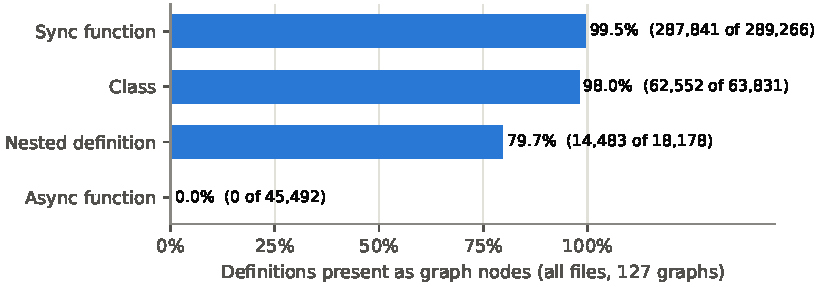
\includegraphics[width=0.78\linewidth]{p1_presence.pdf}
\caption{Share of definitions in every snapshot that exist as graph nodes, by kind. Async functions are absent from all 127 graphs.}
\label{fig:presence}
\end{figure}

Figure~\ref{fig:presence} gives presence by kind. Restricted to non-test source files, sync functions are 100\% present and async functions 0 of 28,113. The missing classes and sync functions are id-scheme effects that the reconciliation accounts for in full: fastapi lists 1,683 inner pydantic \code{Config} classes without their model class, and requests lists a subset of test methods without their test class. Every missing nested definition in fastapi is itself async, as is every one in rich except a single class defined inside a test function; in requests a further 340 are methods of helper classes defined inside test functions.

The omission falls on the code that needs fixing. Of 711 gold-patch symbols, 81 are async and none is a node; one appears present only because the nested async \code{FastAPI.setup.<locals>.openapi} flattens to the id of a different, sync method, \code{FastAPI.openapi}. Overall 470 of 711 gold symbols (66.1\%, CI 62.6 to 69.5) are nodes. 22 tasks have an async gold symbol, 21 of them in fastapi, which is 31\% of fastapi tasks. In 3 usable tasks a gold function that the failing test executes has no node at all. fastapi is an async web framework, and for its request-handling path the graph is silent.

\subsection{The resolver turns omissions into wrong answers}\label{sec:resolver}

\begin{figure}[t]
\centering
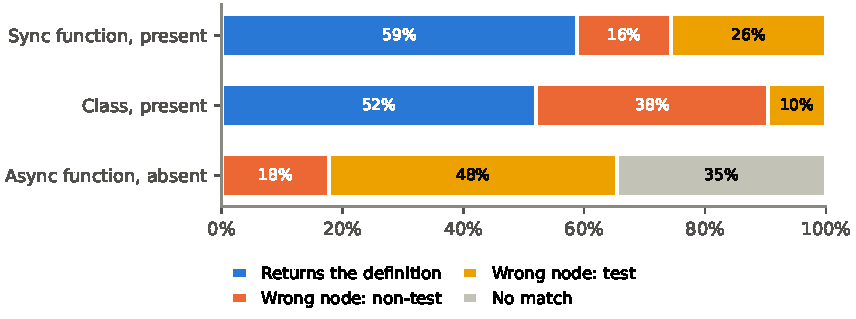
\includegraphics[width=0.78\linewidth]{p1_resolver.pdf}
\caption{What the harness resolver returns for a bare-name query: 287,841 present sync functions, 62,552 present classes, 56,487 absent async functions.}
\label{fig:resolver}
\end{figure}

An agent that asks for an absent function does not get ``not found'' (Figure~\ref{fig:resolver}). For a bare-name query on an absent async function, the resolver returns a different node in 65.4\% of 56,487 cases, a test node in 26,851 of them, and nothing in the remaining 34.6\%. The problem is not limited to absent code: for sync functions that \emph{are} nodes, the bare name resolves to a different, same-named node 41.2\% of the time (46.6\% in fastapi, 62.0\% in httpx), and 47.9\% for classes, because the tie-break prefers short ids and fastapi's tutorial and test modules reuse names. For 21 of 129 tasks, the most specific query for some gold symbol lands on the wrong node.

\subsection{The \texttt{calls} edges against execution}\label{sec:recall}

\begin{table}[t]
\centering\small
\begin{tabular}{lrr}
\toprule
Usable tasks (91) & Value & 95\% CI\\
\midrule
Representable recall & 37.1\% (8,032 of 21,653) & 34.8 to 40.2\\
Agent-facing recall & 31.8\% (8,032 of 25,267) & 29.4 to 34.8\\
Recall on gold-incident calls & 56.3\% (604 of 1,073) & 39.3 to 68.4\\
Observed precision & 21.4\% (8,013 of 37,433) & 20.0 to 22.8\\
\bottomrule
\end{tabular}
\caption{The provided \texttt{calls} edges against calls observed while the tasks' tests run.}
\label{tab:recall}
\end{table}

\begin{figure}[t]
\centering
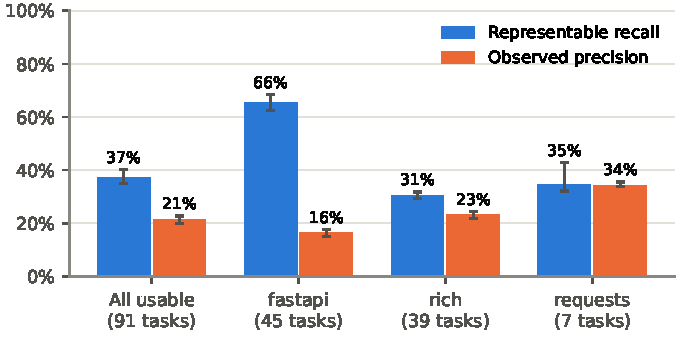
\includegraphics[width=0.72\linewidth]{p1_recall_precision.pdf}
\caption{Representable recall and observed precision, pooled and per repository, with 95\% task-cluster bootstrap intervals.}
\label{fig:recall}
\end{figure}

Table~\ref{tab:recall} and Figure~\ref{fig:recall} give the comparison. Of the observed calls the graph misses, 79\% run between two existing nodes, 11\% touch an omitted sync definition, 6\% a nested function and 4\% an absent async function. Recall is 65.6\% in fastapi, 30.5\% in rich and 34.7\% in requests; precision is lowest in fastapi (16.5\%) and highest in requests (34.3\%). The tests executed 16.7\% of non-test nodes, so all figures describe the code paths the tasks exercise.

This contradicts our hypothesis that the graph would be precise but incomplete, like conservative static analysers~\cite{pycg}: it is incomplete \emph{and} most of its edges between executed functions never ran.

\subsection{What the \texttt{calls} relation encodes}\label{sec:semantics}

\begin{figure}[t]
\centering
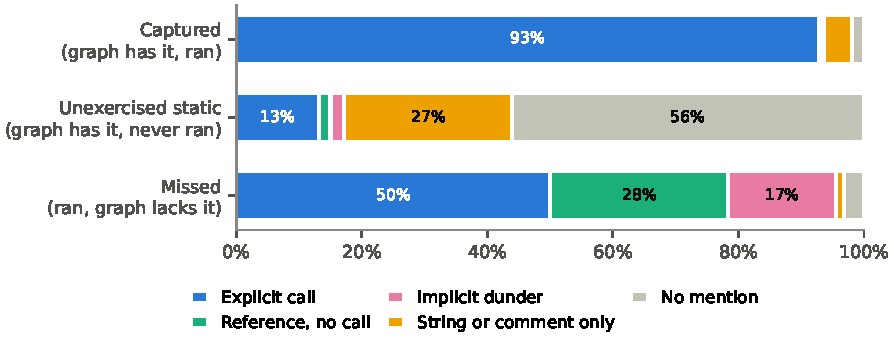
\includegraphics[width=0.8\linewidth]{p1_edge_semantics.pdf}
\caption{How the callee appears in the caller's own source, for non-test edges: 7,640 captured, 35,017 unexercised static, 12,231 missed.}
\label{fig:semantics}
\end{figure}

\begin{figure}[t]
\centering
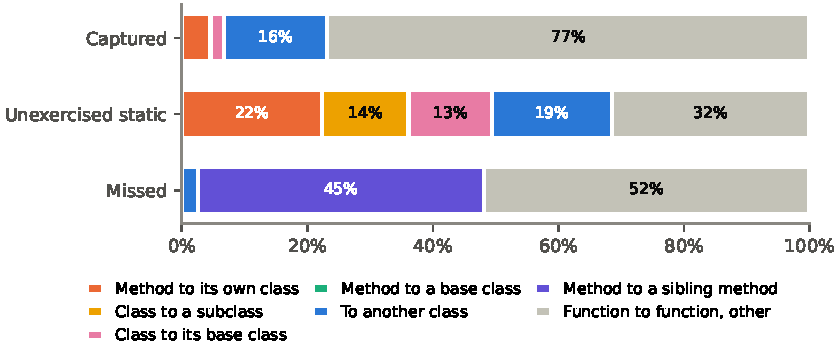
\includegraphics[width=0.8\linewidth]{p1_edge_structure.pdf}
\caption{Structural relation between the endpoints of every non-test edge in the three populations of Figure~\ref{fig:semantics}.}
\label{fig:structure}
\end{figure}

Reading the caller's source explains both numbers (Figure~\ref{fig:semantics}). Captured edges have an explicit call site 88.6\% of the time, mostly bare calls (55.3\%) and instantiations (19.0\%): what a name-matching walker finds. Missed calls are method dispatch that the walker does not resolve: calls on other objects (23.4\%), \code{self.} calls (15.9\%), references passed as callbacks (28.3\%) and implicit dunder calls (17.3\%). The 35,017 unexercised edges mostly have no textual basis in the caller: in 56.1\% the callee is not mentioned at all and in 26.7\% only in a string or comment.

Figure~\ref{fig:structure} shows what they are instead. Of all unexercised non-test edges, 22.3\% point from a method to its own class, 13.8\% from a class to a subclass and 13.3\% from a class to a base class; among missed calls, 45.5\% run between two methods of the same class. We infer that the generator stores containment and inheritance, in both directions, under the label \texttt{calls}, which also explains why 8 to 21\% (30\% in the single httpx graph) of \texttt{calls} edges per graph point from a symbol to its own member. An agent following ``callers'' and ``callees'' is in part walking a class hierarchy.

\subsection{The graph connects failing tests to the fix}\label{sec:reach}

\begin{figure}[t]
\centering
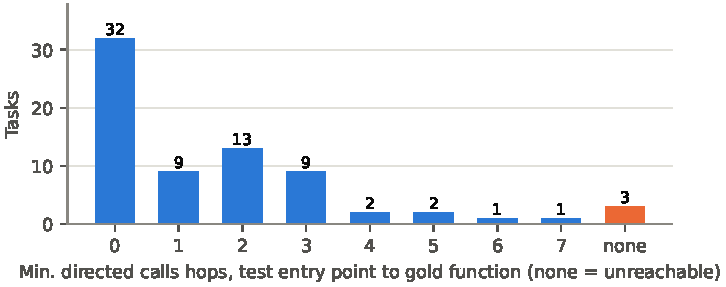
\includegraphics[width=0.76\linewidth]{p1_hops.pdf}
\caption{Minimum directed \texttt{calls} hops from where the failing tests enter the library to a gold function they execute (72 usable tasks with an executed gold node).}
\label{fig:hops}
\end{figure}

Despite the mislabelled and missing edges, the graph does link the code a failing test touches to the code that must change. An entry set exists for 86 of 91 usable tasks, and 72 tasks have a gold function that the failing tests execute and that is a node. In 69 of these 72 (95.8\%, CI 88.5 to 98.6) every such gold function is reachable from the entry set along directed \texttt{calls} edges; none is reachable only against edge direction. Figure~\ref{fig:hops} gives the distances: the gold function is itself an entry point in 32 tasks and within three hops in 63.

We had hypothesized that gold functions would often be reachable at runtime but not in the static graph. On this data the hypothesis is rejected. The obstacles for an agent are omission (async code is absent and cannot be reached), mislabelling (much of a node's frontier is class structure) and distance on a hub-heavy graph, not missing connectivity.

\subsection{Embeddings and retrieval}\label{sec:embed}

\paragraph{The encoder is not public EmbeddingGemma.} No candidate approaches identification: the best mean cosine to the provided vectors is 0.073 for EmbeddingGemma 300m (name variant, document prompt), 0.015 for EmbeddingGemma~2 and 0.036 for the MiniLM control, with pairwise rank correlation at most 0.17 for either EmbeddingGemma (0.21 for the control). The provided vectors are not unit-normalised and are strongly anisotropic: mean cosine to the mean vector is 0.87 to 0.95, the first principal component explains 44\% to 75\% of the variance, and the top-1 neighbour cosine averages 0.999.

\begin{figure}[t]
\centering
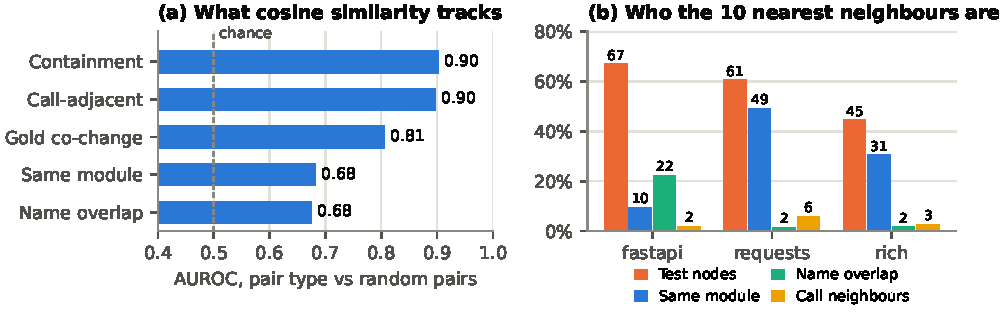
\includegraphics[width=\linewidth]{p1_embeddings.pdf}
\caption{(a) Mean AUROC over 127 graphs for separating each pair type from random pairs by cosine. (b) Composition of each node's 10 nearest neighbours.}
\label{fig:embed}
\end{figure}

\paragraph{What similarity tracks.} Cosine separates containment and call-adjacent pairs from random pairs well (AUROC 0.90), gold co-change pairs less (0.81), same-module and name-overlap pairs weakly (0.68; Figure~\ref{fig:embed}a). But a node's ten nearest neighbours are 45\% to 67\% test nodes and only 2\% to 6\% call neighbours (Figure~\ref{fig:embed}b), so the tool mostly returns tests.

\begin{figure}[t]
\centering
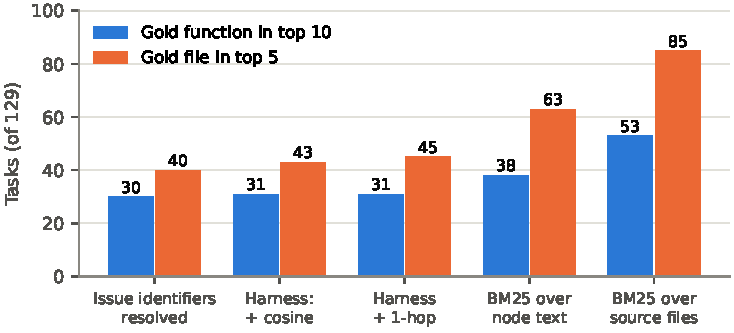
\includegraphics[width=0.78\linewidth]{p1_retrieval.pdf}
\caption{Tasks (of 129) where each mode ranks a gold function in its top 10 or a gold file in its top 5.}
\label{fig:retrieval}
\end{figure}

\paragraph{Retrieval.} Figure~\ref{fig:retrieval} compares the five modes over all 129 tasks. The cosine step changes three tasks and one-hop expansion two more. Free-text BM25 over the source finds the gold file in 47 tasks where the harness mode does not, and the reverse holds for 5 (exact McNemar $p<0.0001$). The harness mode returns nothing for 54 of 129 tasks, because no identifier in the issue resolves to a node.

\section{Released resources}\label{sec:release}
\begin{itemize}
\item \textbf{Audit toolkit}: every step above, with a synthetic-fixture test suite (15 tests).
\item \textbf{Typed graph v2} per base commit, in the harness's format and ids: functions \emph{including async}, nested definitions, and typed edges \texttt{contains}, \texttt{imports}, \texttt{inherits}, \texttt{calls\_static}, \texttt{calls\_dynamic} (with test provenance) and \texttt{tests}.
\item \textbf{Per-task profile}: gold coverage, async exposure, resolver hazards, entry distance, reachability, recall and precision.
\end{itemize}

\section{Implications and limitations}

\paragraph{For agent builders.} Treat \code{get_code_neighbors} output as a mix of call and class-structure edges, check the id a resolved name returns, and use text search for async code; a sandbox Skill script can serve the typed graph legally.

\paragraph{For benchmark designers.} Document the graph's semantics, split containment, inheritance and calls into typed edges, return ``not found'' instead of a substring match, and include async definitions.

\paragraph{Limitations.} Precision is a lower bound measured only inside executed code. Our runs used per-task environments with network access rather than the official cached dependencies; 9 collection errors, 2 import errors and 4 requests tasks without collectable tests are our setup, not the tasks. Recall covers the paths the tests exercise. The generator's rules are inferred from its outputs, and the 80-edge hand-review sample is not yet labelled. The hidden test set uses the same generator, but we have not measured it. Results come from four repositories, two of which dominate the task count.

\section*{Reproducibility}
Every number comes from result files under \code{planA_results/vm-a2/results/} (\code{a1_v2}, \code{a7}, \code{a2_v3}, \code{a8}, \code{a3}, \code{a5_v3}, \code{a6_v3}) and \code{vm-main/results/a4}. \code{scripts/ops/} regenerates them from the competition archive; \code{papers/make_figures.py} draws every figure.

\begin{thebibliography}{99}\small
\bibitem{pycg} V.~Salis et al. PyCG: Practical call graph generation in Python. ICSE, 2021. \url{https://consensus.app/papers/details/b2f145e1fe035745a8b387e3f4b74740/}
\bibitem{infercg} Y.~Xiang et al. InferCG: Enhancing Python call graph generation via static analysis and LLMs. TOSEM, 2026. \url{https://consensus.app/papers/details/f9176ef478f6583eaef6c696919949a8/}
\bibitem{kummita} S.~Kummita et al. Qualitative and quantitative analysis of callgraph algorithms for Python, 2021. \url{https://consensus.app/papers/details/2565e0e7f78a5d05b74121697239f917/}
\bibitem{sui} L.~Sui et al. On the recall of static call graph construction in practice. ICSE, 2020. \url{https://consensus.app/papers/details/93f20309e7855a5898b1f0f293a01442/}
\bibitem{helm} D.~Helm et al. Total recall? How good are static call graphs really? ISSTA, 2024. \url{https://consensus.app/papers/details/c62e543287615a7abeb7430f76391389/}
\bibitem{codeanchor} Lin et al. How much static structure do code agents need? (CodeAnchor). ISSTA, 2026. \url{https://www.alphaxiv.org/abs/2606.26979}
\bibitem{larger} Hu et al. LARGER: Lexically anchored repository graph exploration and retrieval, 2026. \url{https://www.alphaxiv.org/abs/2605.16352}
\bibitem{semnav} Wei et al. SemNav: Semantic navigation for repository-level issue localization, 2026. \url{https://www.alphaxiv.org/abs/2609.31176}
\bibitem{codecompass} Paipuru. The navigation paradox in large-context agentic coding (CodeCompass), 2026. \url{https://www.alphaxiv.org/abs/2602.20048}
\bibitem{daira} Liu et al. DAIRA: Dynamic analysis-enhanced issue resolution agent, 2026. \url{https://www.alphaxiv.org/abs/2603.22048}
\bibitem{grepo} Wang et al. GREPO: A benchmark for GNNs on repository-level bug localization, 2026. \url{https://www.alphaxiv.org/abs/2602.13921}
\bibitem{graphlocator} Liu et al. GraphLocator: Graph-guided causal reasoning for issue localization, 2025. \url{https://www.alphaxiv.org/abs/2512.22469}
\bibitem{caumartin} Caumartin et al. Retrieval-oriented code representations in agentic bug localization, 2026. \url{https://www.alphaxiv.org/abs/2607.11046}
\bibitem{smallagents} Lasbordes et al. Small agents with semantic search: Efficient multilingual code localization, 2026. \url{https://www.alphaxiv.org/abs/2610.05099}
\bibitem{eg2} Google DeepMind. EmbeddingGemma 2 model card, 2026. \url{https://huggingface.co/google/embeddinggemma-2}
\bibitem{gemma4} Gemma Team. Gemma 4 technical report, 2026. \url{https://www.alphaxiv.org/abs/2607.02770}
\bibitem{overreliance} Yang et al. Agents' overreliance on unreliable tools, 2026. \url{https://www.alphaxiv.org/abs/2609.05587}
\end{thebibliography}

\end{document}
